As Dennard scaling ends, big-data applications such as real-time image processing, graph analytics, and deep learning continue to push the boundaries of performance and energy efficiency requirements for computing system. 
One solution to this challenge is to move compute closer to memory or storage for substantial energy savings of data movement. 
We have developed an innovative Near-Data Computing (NDC) architecture that leverages the dramatic opportunities provided by the new CXL protocol \cite{sharma2020compute}. 
NDC incorporates heterogenous compute elements in the memory/storage subsystem to accelerate various computing tasks near data. 
One of these compute elements is the Streaming Engine (SE).

The SE is a Coarse-Grained Reconfigurable Array (CGRA) that is composed of interconnected compute tiles.  
The compute tiles are interconnected with both a Synchronous Fabric (SF) and an Asynchronous Fabric (AF) as shown in Fig. \ref{fig:sub-se}.
It also interconnects tile memory, multiplexers, and Single Instruction Multiple Data (SIMD) units within each tile as shown in Fig. \ref{fig:sub-tile}. 
Tiles can be pipelined through SF to form a Synchronous Data Flow (SDF) through Multiply/Shift (MS) unit and an Arithmetic/Logic (AL) SIMD units. 
The output of the MS unit is connected to one of the two inputs of the AL unit.
AF connects a tile with all other tiles, dispatch interface (DI), and memory interfaces (MI).
It bridges SDFs through asynchronous operations, which include SDF initiation, asynchronous data transfer from one SDF to another, system memory accesses, and branching and looping constructs. 
Together, SF and AF allow the tiles to efficiently execute high-level programming language constructs.
Simulation results of hand-crafted SE kernels have shown orders-of-magnitude better performance per watt on data-intensive applications than existing computing platforms.

\begin{figure}
  \centering
  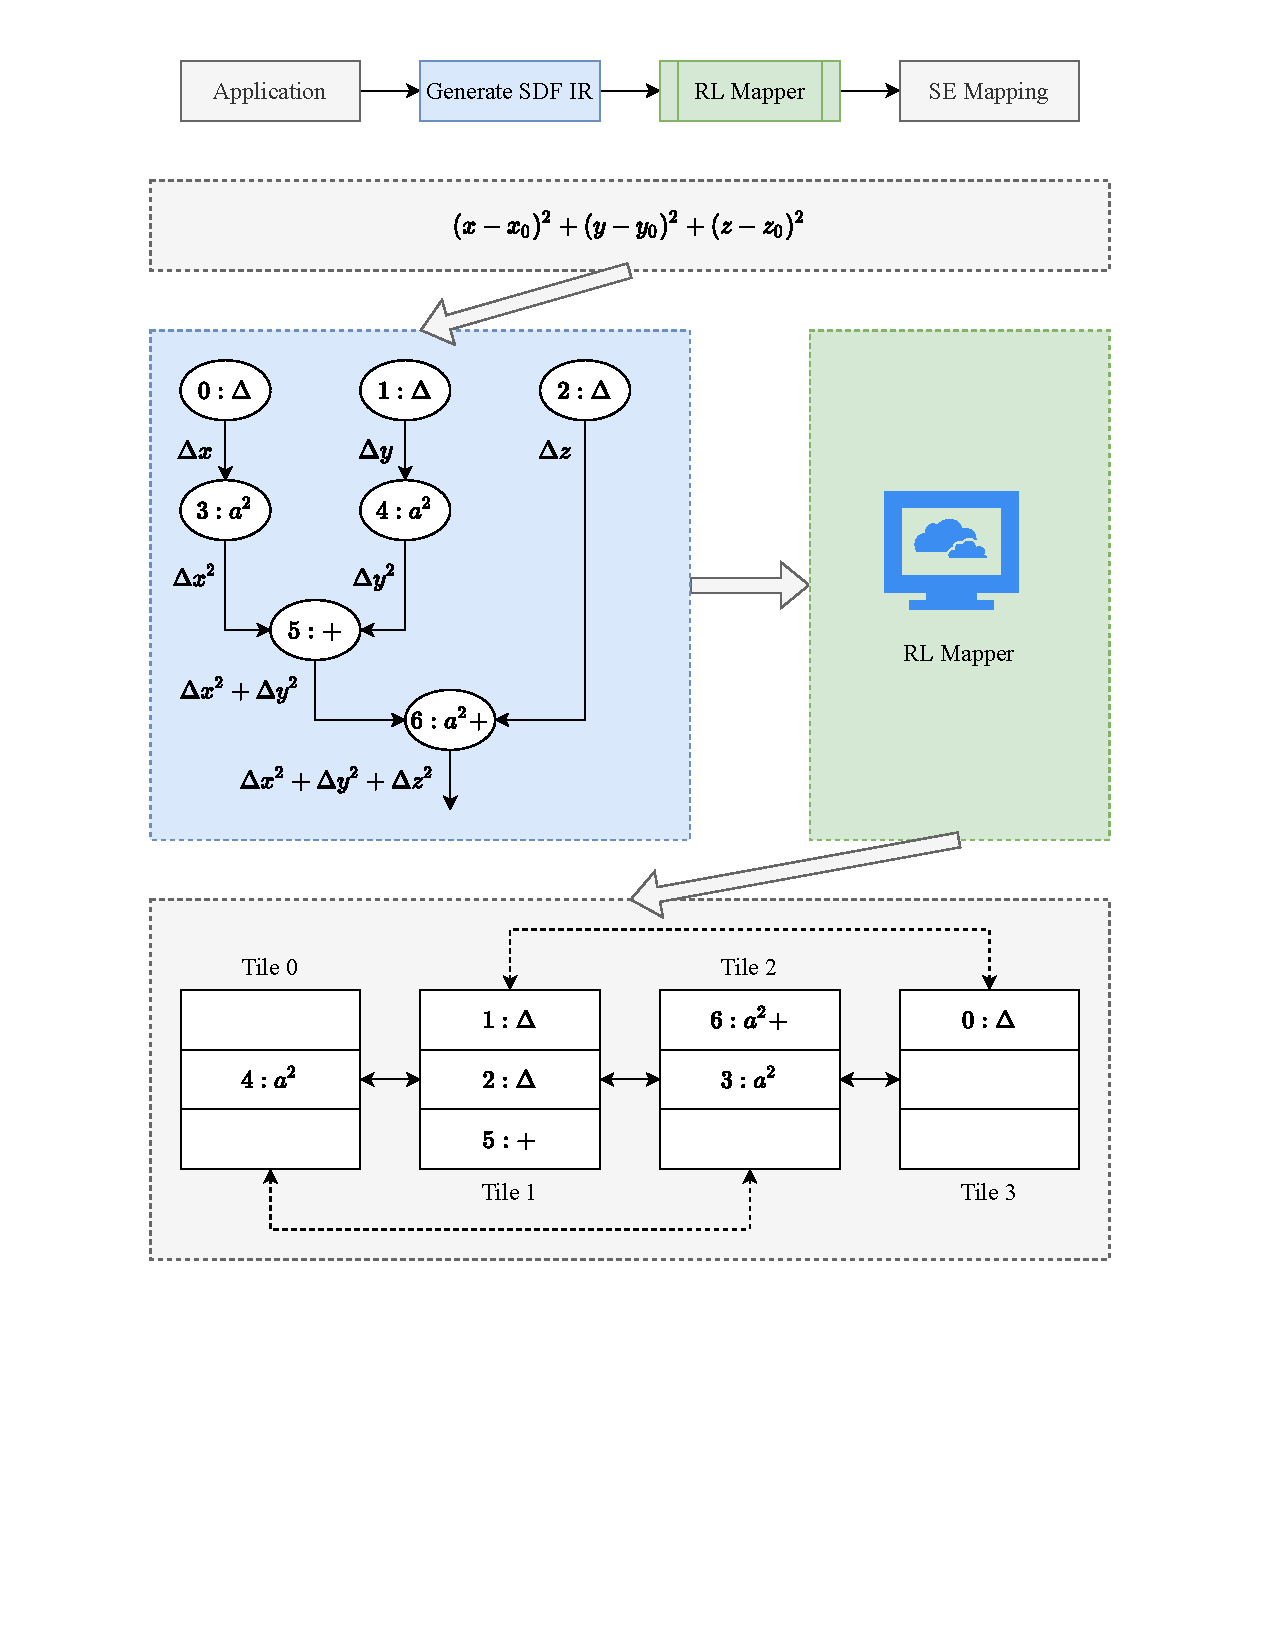
\includegraphics[trim=70 180 70 25, clip, width=\linewidth]{fig/SE_example.pdf}
  \caption{
    Example showing a mapping of a distance calculation function onto the SE device.
    The instruction execution latency is three clock cycles.
    The solid and dotted lines connecting the tiles, have one and two clock cycles transfer latency respectively.
    E.g., instruction \#0 is scheduled at (tile \#3, slot \#0) and its output is sent to instruction \#3.
    Instruction \#0 output is ready after three clock cycles plus two clock cycles to move data to tile \#1. 
    Thus, instruction \#3 gets scheduled on (tile \#1, slot \#1).
  }
  \label{fig:se_example}
\end{figure}

A simple example that illustrates a program mapped to the SE is shown in \figurename~\ref{fig:se_example}.
The program in this example is a distance calculation function shown in Eq. \ref{eq:dist}.

\begin{equation}
    \label{eq:dist}
    D = \sqrt{(x - x_0)^2 +(y - y_0)^2 + (z - z_0)^2}
\end{equation}

To keep this example simple, we ignore the square root part of the equation.
The program is represented as SDF as shown in \figurename~\ref{fig:se_example}.
Each operation in Eq. \ref{eq:dist} is an instruction that is mapped to a slot at a tile on the SE.

Since the output of the MS unit is connected to the input of the AL unit, instruction \#6 produces $\Delta z^2$ on the output on the MS unit and adds it to $(\Delta x^2 + \Delta y^2)$ at the AL unit.

Mapping the instructions from a program's SDF onto the compute elements of the SE while adhering to architectural constraints is an NP-hard problem with a vast and sparse search space \cite{10.1007/3-540-69346-7_30}. 
Constraints related to tile memory, synchronous dataflow, the use of delays to match timing requirements and more are necessary to ensure correct execution. 
Creating the mappings manually or using brute force algorithms takes time and lots of effort even for the simplest of programs. 
This process also adds assumptions that reduce the search space, trading off optimization possibilities.  

In this work we propose a deep Reinforcement Learning (RL) method to explore and find optimal mappings in an unsupervised manner. 
Using the Proximal Policy Optimization (PPO) method we train a neural network model to place instructions onto the SE tiles guided by a reward function in an environment that models the SE device and its constraints. 
We also present Global Graph Attention (GGA) module that improves the baseline feedforward models by providing attention mechanism to the RL model.
Our RL method is combined with output masking, finetuning and sorted iteration order, which will be presented in the following sections.

The trained model is able to create valid mappings for the SE by learning about the structure of the problem domain.
On average addition of GGA finds 10\% better instruction schedules in terms of clock cycles for varying graphs complexities and different SE device configurations.

The key contributions of this paper are as follows:
\begin{enumerate}
    \item A Reinforcement Learning methodology that is able to map the instructions from a given SDF to the processing elements in the SE and has the potential to be reused across SDF graphs.
    \item An analysis of different factors that impacts the quality of mappings obtained, such as attention module, output masking and iteration order.
\end{enumerate}

This work is motivated by the need to provide an improved SE toolset that lowers the SE usability barrier for a programmer.
In addition, the proposed mapper can be used along with other SE tools or assist in the manual mapping of applications to the SE by providing partial placement suggestions or tile configuration labels.
The RL mapper performs unsupervised learning and optimization allowing it to search a wide and sparse search space. 
Each node in the SDF is an instruction that is mapped to a specific slot on a tile.

This line of research is inspired by recent work that used RL for chip placement \cite{mirhoseini2020chip}.
The problem requirement of mapping nodes of a SDF to available compute elements is similar to the problem of placing nodes of a chip netlist on a chip canvas. 
% Due to the similarities between these problem domains, we theorize that our approach has the potential of being used for chip placement.
% This hypothesis will be investigated in future work.

The rest of this paper is organized as follows: 
Section \ref{sec:relatedwork} discusses related work.
Section \ref{sec:background} provides the necessary background on the SE device architecture needed to understand the details of the RL approach.
Section \ref{sec:rlmapper} presents the proposed RL approach for mapping applications to the SE.
Section \ref{sec:results} discusses results, and Section \ref{sec:conclusion} concludes the paper along with a discussion on future work.